
% This LaTeX was auto-generated from an M-file by MATLAB.
% To make changes, update the M-file and republish this document.

\documentclass{article}
\usepackage{graphicx}
\usepackage{color}
\usepackage{listings}
\usepackage[framed]{mcode}
\usepackage{fullpage}
\usepackage{amsmath}
\usepackage[utf8x]{inputenc}
\usepackage{import}
\usepackage{setspace}
\usepackage{hyperref}
\definecolor{lightgray}{gray}{0.5}
\setlength{\parindent}{0pt}

\begin{document}

    
    
%\section*{}

 \title{BE 521: Homework 4 \\{\normalsize HFOs}
\\{\normalsize Spring 2021}} \author{58 points} \date{Due: Tuesday,
2/23/2021 10:00pm} \maketitle \textbf{Objective:} HFO detection and
cross-validation 
 \begin{center} \author{Jal Mahendra Panchal}
\end{center}


\subsection*{HFO Dataset} High frequency oscillations (HFOs) are
quasi-periodic intracranial EEG transients with durations on the
order of tens of milliseconds and peak frequencies in the range of
80 to 500 Hz. There has been considerable interest among the
epilepsy research community in the potential of these signals as
biomarkers for epileptogenic networks.\\\\
In this homework exercise, you will explore a dataset of candidate
HFOs detected using the algorithm of Staba et al. (see article on
Canvas). The raw recordings from which this dataset arises come from
a human subject with mesial temporal lobe epilepsy and were
contributed by the laboratory of Dr. Greg Worrell at the Mayo Clinic
in Rochester, MN.\\\\
The dataset \verb|I521_A0004_D001| contains raw HFO clips that are
normalized to zero mean and unit standard deviation but are
otherwise unprocessed. The raw dataset contain two channels of data:
\verb|Test_raw_norm| and \verb|Train_raw_norm|, storing raw testing
and training sets of HFO clips respectively. The raw dataset also
contains two annotation layers: \verb|Testing windows| and
\verb|Training windows|, storing HFO clip start and stop times (in
microseconds) for each of the two channels above.
Annotations contain the classification by an ``expert'' reviewer
(i.e., a doctor) of each candidate HFO as either an HFO (2) or an
artifact (1). On ieeg.org and upon downloading the annotations,
You can view this in the "description" field. \\\\
After loading the dataset in to a \verb|session| variable as in
prior assignments you will want to familiarize yourself with the
\verb|IEEGAnnotationLayer| class. Use the provided "getAnnotations.m"
function to get all the annotations from a given dataset. The first
output will be an array of annotation objects, which you will see
also has multiple fields including a description field as well as start and stop times. Use
You can use the information outputted by getAnnotations to pull
each HFO clip.


\section{Simulating the Staba Detector (12 pts)} Candidate HFO clips
were detected with the Staba et al. algorithm and subsequently
validated by an expert as a true HFO or not. In this first section,
we will use the original iEEG clips containing HFOs and re-simulate
a portion of the Staba detection.
\begin{enumerate}
    \item How many samples exist for each class (HFO vs artifact) in
    the training set? (Show code to support your answer) (1 pt).\\


\textbf{Answer 1.1:}

\begin{lstlisting}
%Fetch I521_A0004_D001 data
addpath(genpath('/Users/jalpanchal/git/be521'));

session_hfo = IEEGSession('I521_A0004_D001', 'jalpanchal', 'jal_ieeglogin.bin');
sampling_frequency_hz_hfo = session_hfo.data.sampleRate;
duration_in_sec_hfo = session_hfo.data(1).rawChannels(1).get_tsdetails.getDuration/1e6;

test_raw_norm = session_hfo.data.getvalues(0, duration_in_sec_hfo * 1e6, 1);
train_raw_norm = session_hfo.data.getvalues(0, duration_in_sec_hfo * 1e6, 2);

datestr(seconds(duration_in_sec_hfo),'HH:MM:SS:FFF')
\end{lstlisting}

\color{lightgray} \begin{lstlisting}IEEGSETUP: Adding 'ieeg-matlab.jar' to dynamic classpath
Warning: Objects of
edu/upenn/cis/db/mefview/services/TimeSeriesDetails
class exist - not clearing java 
Warning: Objects of
edu/upenn/cis/db/mefview/services/TimeSeriesInterface
class exist - not clearing java 
IEEGSETUP: Found log4j on Java classpath.
URL: https://www.ieeg.org/services
Client user: jalpanchal
Client password: ****

ans =

    '00:00:09:466'

\end{lstlisting} \color{black}


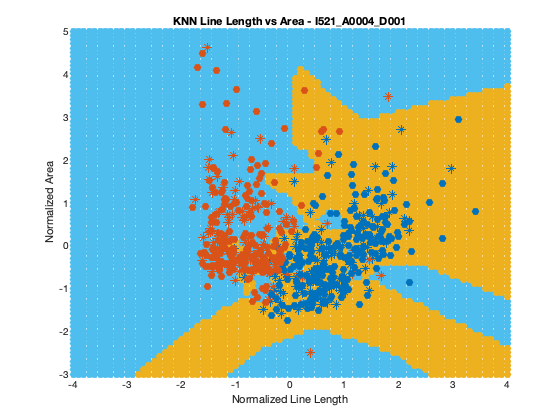
\includegraphics [width=5in]{jalp_hw4_01.png}
\begin{lstlisting}
%Get annotations
dataset = session_hfo.data;
layerName = 'Training windows';
[allEvents, timesUSec, channels] = getAnnotations(dataset,layerName);
\end{lstlisting}
\begin{lstlisting}
%parsing description and event timing and time series
train_data = {str2double(allEvents(1).description), allEvents(1).start,...
               allEvents(1).stop, session_hfo.data.getvalues(allEvents(1).start, allEvents(1).stop-allEvents(1).start, 2)};
for i = 2:size(allEvents,2)
    train_data = [train_data;{str2double(allEvents(i).description),...
        allEvents(i).start, allEvents(i).stop, ...
        session_hfo.data.getvalues(allEvents(i).start, allEvents(i).stop-allEvents(i).start, 2) }];
end
\end{lstlisting}
\begin{lstlisting}
hfo_train = find(cell2mat(train_data(:, 1))==2);
artif_train = find(cell2mat(train_data(:, 1))==1);

number_hfo_training = size(hfo_train, 1)
number_artifact_training =  size(artif_train,1)
\end{lstlisting}

\color{lightgray} \begin{lstlisting}
number_hfo_training =

   101


number_artifact_training =

    99

\end{lstlisting} \color{black}
The number of samples for HFO is 101 and that for artifacts is 99.

    \item Using the training set, find the first occurrence of the
    first valid HFO and the first artifact.
        Using \verb|subplot| with 2 plots, plot the valid HFO's
        (left) and artifact's (right) waveforms. Since the units are
        normalized, there's no need for a y-axis, so remove it with
        the command \verb|set(gca,'YTick',[])|. (2 pts).\\


\textbf{Answer 1.2:}

\begin{lstlisting}
%test_raw_norm = session_hfo.data.getvalues(0, duration_in_sec_hfo * 1e6, 1);
%fetching first occurance of HFO
i= 1;
fs = sampling_frequency_hz_hfo;
t_hfo = train_data{hfo_train(i),2}/1e3 : 1e3/fs : train_data{hfo_train(i),3}/1e3;
hfo_1_train = train_data{hfo_train(i), 4};

%fetching first occurance of artifact
t_artif = train_data{artif_train(i),2}/1e3 : 1e3/fs : train_data{artif_train(i),3}/1e3;
artif_1_train = train_data{artif_train(i), 4};
\end{lstlisting}
\begin{lstlisting}
%plots
figure();
ax1 = subplot(1,2,1);
plot(t_hfo, hfo_1_train, 'Linewidth', 1.5);
title('HFO(1)')
xlabel('Time (ms)')
set(ax1, 'YTick', [])
ax1.Position = [0.1300 0.1100 0.3747 0.8150];

ax2 = subplot(1,2,2);
plot(t_artif, artif_1_train, 'Linewidth', 1.5)
title('Artifact(1)')
xlabel('Time (ms)')
set(ax2, 'YTick', [])
ax2.Position = [0.5303 0.1100 0.3747 0.8150];


suptitle('First samples in training window in I521\_A0004\_D001')
\end{lstlisting}


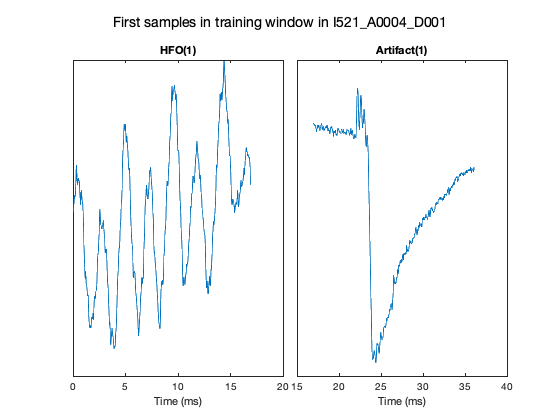
\includegraphics [width=5in]{jalp_hw4_02.png}

    \item Using the \texttt{fdatool} in MATLAB, build an FIR
    bandpass filter of the equiripple type of order 100.
        Use the Staba et al. (2002) article to guide your choice of
        passband and stopband frequency. Once set, go to
        \texttt{File} \verb|->| \texttt{Export}, and export
        ``Coefficients'' as a MAT-File. Attach a screenshot of your
        filter's magnitude response. (Note: We will be flexible with
        the choice of frequency parameters within reason.) (3 pts) \\


\textbf{Answer 1.3:}

FIR Bandpass filter Magnitude response:

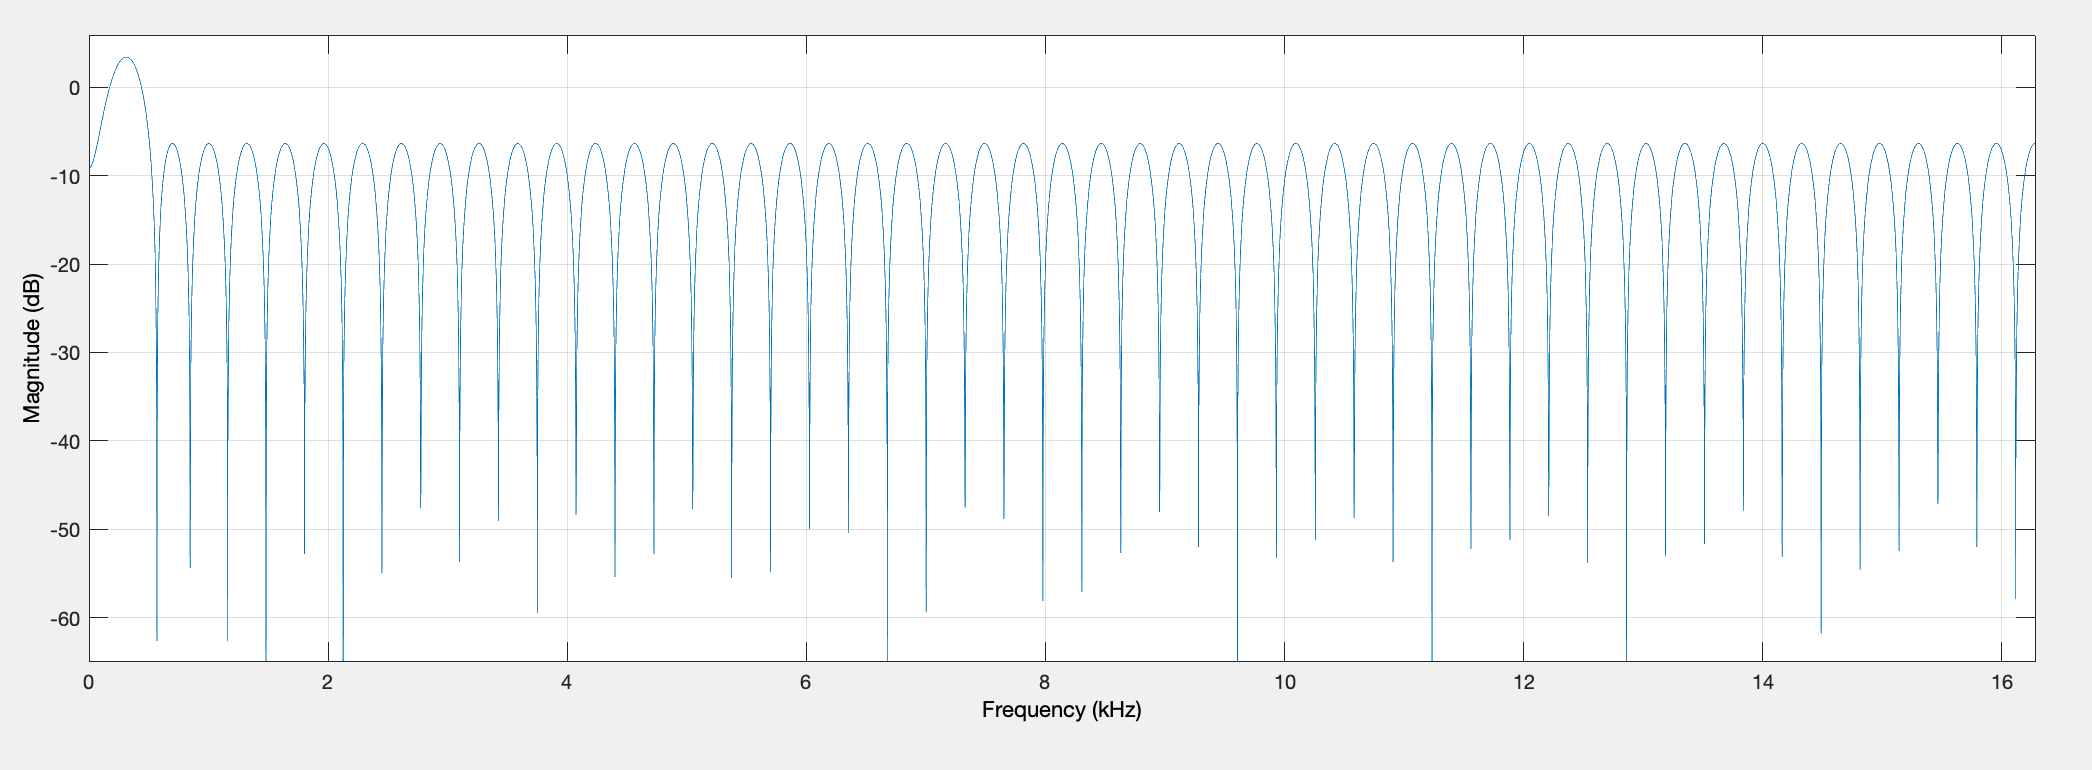
\includegraphics[scale=0.4]{screenshot_p1q3.png}


    \item Using the forward-backward filter function
    (\texttt{filtfilt}) and the numerator coefficients saved above,
        filter the valid HFO and artifact clips obtained earlier.
        You will need to make a decision about the input argument
        \texttt{a} in the \texttt{filtfilt} function. Plot these two
        filtered clips overlayed on their original signal in a two
        plot \texttt{subplot} as before. Remember to remove the
        y-axis. (3 pts) \\


\textbf{Answer 1.4:}

\begin{lstlisting}
load('./fir_staba.mat')
b = fir_b;
a = 1;

hfo_1_filter = filtfilt(b,a,hfo_1_train);
artif_1_filter = filtfilt(b,a,artif_1_train);
\end{lstlisting}
\begin{lstlisting}
%plots
figure();
ax1 = subplot(1,2,1);
plot(t_hfo, hfo_1_train, 'Linewidth', 0.5);
hold on
plot(t_hfo, hfo_1_filter, 'Linewidth', 1.2);
hold off
title('HFO(1)')
xlabel('Time (ms)')
ylim([1.1*min(hfo_1_train), 1.2*max(hfo_1_train)])
legend('raw HFO','filtered HFO', 'Location','northwest')
set(ax1, 'YTick', [])
ax1.Position = [0.1300 0.1100 0.3747 0.8150];

ax2 = subplot(1,2,2);
plot(t_artif, artif_1_train, 'Linewidth', 0.5)
hold on
plot(t_artif, artif_1_filter, 'Linewidth', 1.2)
hold off
title('Artifact(1)')
xlabel('Time (ms)')
ylim([1.1*min(artif_1_train), 1.5*max(artif_1_train)])
legend('raw artifacts','filtered artifacts')
set(ax2, 'YTick', [])
ax2.Position = [0.5303 0.1100 0.3747 0.8150];


suptitle('FIR filter on training data in I521\_A0004\_D001')
\end{lstlisting}


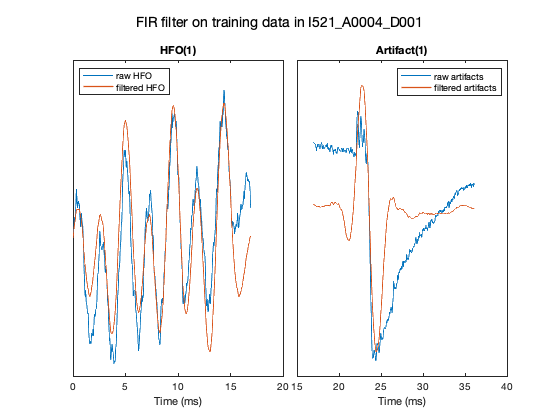
\includegraphics [width=5in]{jalp_hw4_03.png}

    \item Speculate how processing the data using Staba's method may
    have erroneously led to a false HFO detection (3 pts) \\


\textbf{Answer 1.5:}

The processing of data using Staba's method involves using a equiripple bandpass filter. From the image of the filtered artifacts signal above we see that it the original noisy artifact signal has been converted to a sinosoidal signal. Depending on how the HFO detection algorithms work, its peak and profile can very easily be mistaken for a HFO. The filtering of high frequencies and low frequenncy variations and possibly the impact of the filter windows is amplifying mid frequency signals in the filtered artifact signal which looks similar in profile as the valid HFO signals. These reason could cause Staba's method to erroneously lead to false HFO detection.\ensuremath{\backslash}\ensuremath{\backslash}

\end{enumerate}
\section{Defining Features for HFOs (9 pts)} In this section we will
be defining a feature space for the iEEG containing HFOs and
artifacts. These features will describe certain attributes about the
waveforms upon which a variety of classification tools will be
applied to better segregate HFOs and artifacts
\begin{enumerate}
    \item Create two new matrices, \verb|trainFeats| and
    \verb|testFeats|, such that the number of rows correspond to
    observations (i.e. number of training and testing clips)
        and the number of columns is two. Extract the line-length and
        area features (seen previously in lecture and Homework 3) from
        the normalized raw signals (note: use the raw signal from
        ieeg.org, do not filter the signal). Store the line-length value
        in the first column and area value for each sample in the second
        column of your features matrices. Make a scatter plot of the
        training data in the 2-dimensional feature space, coloring the
        valid detections blue and the artifacts red. (Note: Since we only
        want one value for each feature of each clip, you will
        effectively treat the entire clip as the one and only
        ``window''.) (4 pts) \\


\textbf{Answer 2.1:}

\begin{lstlisting}
%First we'll get the time series of each observation for testing set
%Get annotations
dataset = session_hfo.data;
layerName = 'Testing windows';
[allEvents, timesUSec, channels] = getAnnotations(dataset,layerName);
\end{lstlisting}
\begin{lstlisting}
%parsing description and event timing and time series
test_data = {str2double(allEvents(1).description), allEvents(1).start,...
               allEvents(1).stop, session_hfo.data.getvalues(allEvents(1).start, allEvents(1).stop-allEvents(1).start, 1)};
for i = 2:size(allEvents,2)
    test_data = [test_data;{str2double(allEvents(i).description),...
        allEvents(i).start, allEvents(i).stop, ...
        session_hfo.data.getvalues(allEvents(i).start, allEvents(i).stop-allEvents(i).start, 1) }];
end
\end{lstlisting}
\begin{lstlisting}
%Function definition
%LineLength
LLFn = @(x) sum(abs(diff(x)));

%Area
AreaFn = @(x) sum(abs(x));
\end{lstlisting}
\begin{lstlisting}
%Calculating features for training set
trainFeats = zeros(size(train_data,1), 2);

for i = 1:size(train_data,1)
    temp_ =train_data{i,4};
    temp_(isnan(temp_))=0;
    trainFeats(i,1) = LLFn(temp_);
    trainFeats(i,2) = AreaFn(temp_);
end
\end{lstlisting}
\begin{lstlisting}
%Calculating features for testing set
testFeats = zeros(size(test_data,1), 2);

for i = 1:size(test_data,1)
    temp_ =test_data{i,4};
    temp_(isnan(temp_))=0;
    testFeats(i,1) = LLFn(temp_);
    testFeats(i,2) = AreaFn(temp_);
end
\end{lstlisting}
\begin{lstlisting}
%Scatter plot of training data
hfo_train = find(cell2mat(train_data(:, 1))==2);
artif_train = find(cell2mat(train_data(:, 1))==1);

figure();
scatter(trainFeats(hfo_train,1), trainFeats(hfo_train,2), 60,  'filled', 'MarkerFaceColor', [0 0.4470 0.7410])

hold on
scatter(trainFeats(artif_train, 1), trainFeats(artif_train,2), 60, 'filled', 'MarkerFaceColor', [0.8500 0.3250 0.0980])
title('Training set Line Length vs Area - I521\_A0004\_D001')
xlabel('Line Length')
ylabel('Area')
legend('HFOs','artifacts')
\end{lstlisting}


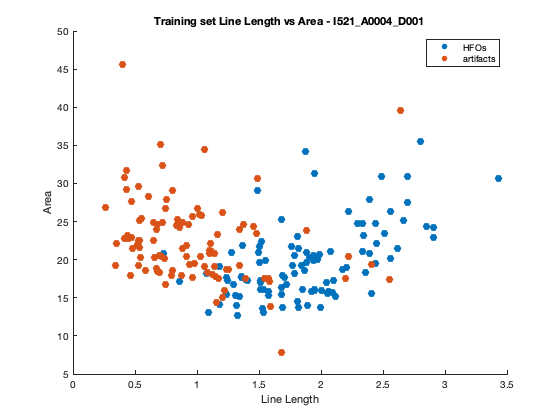
\includegraphics [width=5in]{jalp_hw4_04.png}

    \item Feature normalization is often important. One simple
    normalization method is to subtract each feature by its mean and
    then divide by its standard deviation
        (creating features with zero mean and unit variance). Using
        the means and standard deviations calculated in your
        \emph{training} set features, normalize both the training
        and testing sets. You should use these normalized features for
        the remainder of the assignment.
    \begin{enumerate} \item What is the statistical term for the
    normalized value, which you have just computed? (1 pt) \\


\textbf{Answer 2.2a:}

The statistical term for the normalized value is a \%\ensuremath{\backslash}emph\{Z-score\}\%. It tells us how many standard deviations above or below the mean the given value is.
\begin{lstlisting}
%Calculating normalized feature values
mean_ll_area  = mean(trainFeats);
std_ll_area = std(trainFeats);

trainFeats_norm = (trainFeats-mean_ll_area)./std_ll_area;
testFeats_norm = (testFeats-mean_ll_area) ./std_ll_area;
\end{lstlisting}

	\item Explain why such a feature normalization might be critical
	to the performance of a $k$-NN classifier. (2 pts) \\


\textbf{Answer 2.2b:}

Machine learning algorithms like $k$-NN classifiers can be influenced by the magnitude of different variables during classification. When calculating the distance of the nearest neighbours, the magnitude of the variables will influence the relative distance between points. To avoid such a situation, the variables are normalised using their z-score. The normalized variables now wont have an undue influence due to magnitude on the algorithms like $k$-NN classifiers

\item Explain why (philosophically) you use the training feature means and
	standard deviations to normalize the testing set. (2 pts) \\


\textbf{Answer 2.2c:}

The test set is suppose to represent new unknown data that is used to test how the algorithm will work with new data. In doing so the test data should not influence the normalization of the data as it a new and unknown.\$\ensuremath{\backslash}\ensuremath{\backslash}\$ While at the same time, using the same mean and standard deviation from the training set on the test set means that we are giving the same standardised and uniform treatment to all the data that the algorithm interacts with. This way we allow the intrinsic features of each new data-set to impact its result.

    \end{enumerate}
\end{enumerate}
\section{Comparing Classifiers (20 pts)} In this section, you will
explore how well a few standard classifiers perform on this dataset.
Note, the logistic regression, $k$-NN, and SVM classifiers are functions
built into some of Matlabs statistics packages. If you don't have
these (i.e., Matlab doesn't recognize the functions), and you are
experiencing any difficulty downloading the necessary packages, please
let us know.
\begin{enumerate}
 \item Using Matlab's logistic regression classifier function,
 (\texttt{mnrfit}), and its default parameters, train a model on the
 training set. Using Matlab's \texttt{mnrval} function, calculate
 the training error (as a percentage) on the data. For extracting
 labels from the matrix of class probabilities, you may find the
 command \texttt{[$\sim$,Ypred] = max(X,[],2)} useful\footnote{Note:
 some earlier versions of Matlab don't like the \texttt{$\sim$},
 which discards an argument, so just use something like
 \texttt{[trash,Ypred] = max(X,[],2)} instead.}, which gets the
 column-index of the maximum value in each row (i.e., the class with
 the highest predicted probability). (3 pts) \\


\textbf{Answer 3.1:}

\begin{lstlisting}
%Logistic Regression Classifier
X = trainFeats_norm;
Y = cell2mat(train_data(:,1));

%logistic regression
[B,dev,stat] = mnrfit(X,Y);

%calculating predicted probalities
pihat = mnrval(B,X);
[~, Ypred_train_mnr] = max(pihat, [],2);

%Calculating training error
train_error_mnr = size(find(Ypred_train_mnr~=Y),1)/size(Y,1)
\end{lstlisting}

\color{lightgray} \begin{lstlisting}
train_error_mnr =

    0.1250

\end{lstlisting} \color{black}
The error in training is 12.5\%

 \item Using the model trained on the training data, predict the
 labels of the test samples and calculate the testing error. Is the
 testing error larger or smaller than the training error? Give one
 sentence explaining why this might be so. (2 pts) \\


\textbf{Answer 3.2:}

\begin{lstlisting}
%calculating predicted probalities for testing set
X = testFeats_norm;
Y_test = cell2mat(test_data(:,1));
pihat = mnrval(B,X);
[~, Ypred_test_mnr] = max(pihat, [],2);

%Calculating training error
test_error_mnr = size(find(Ypred_test_mnr~=Y_test),1)/size(Y_test,1)
\end{lstlisting}

\color{lightgray} \begin{lstlisting}
test_error_mnr =

    0.1333

\end{lstlisting} \color{black}
Using the trained model on the testing data, we get an error of 13.33\%.\%\ensuremath{\backslash}\ensuremath{\backslash}\% Which is a little higher than the testing error. This is expected as the model was fit in using the training data so that coefficients of the weights are more tuned to the training set as compared to the testing set. Since the testing set has new data that more likely wil not have that same composition as the traning set we would observe a slightly higher error realistically.

 \item
  \begin{enumerate}
   \item Use Matlab's $k$-nearest neighbors function,
   \texttt{fitcknn}, and its default parameters ($k$ = 1, among
   other things), calculate the training and testing errors. (3 pts) \\


\textbf{Answer 3.3a:}

\begin{lstlisting}
%K nearest neighbor classifier
X = trainFeats_norm;
Y = cell2mat(train_data(:,1));

knn = fitcknn(X,Y, 'NumNeighbors', 1)
\end{lstlisting}

\color{lightgray} \begin{lstlisting}
knn = 

  ClassificationKNN
             ResponseName: 'Y'
    CategoricalPredictors: []
               ClassNames: [1 2]
           ScoreTransform: 'none'
          NumObservations: 200
                 Distance: 'euclidean'
             NumNeighbors: 1


\end{lstlisting} \color{black}
\begin{lstlisting}
%Calculating training error by predicting the training set
Ypred_train_knn = predict(knn, X);

train_error_knn = size(find(Ypred_train_knn~=Y),1)/size(Y,1)
\end{lstlisting}

\color{lightgray} \begin{lstlisting}
train_error_knn =

     0

\end{lstlisting} \color{black}
\begin{lstlisting}
%Calculating testing error using the trained knn model
X  = testFeats_norm;
Y_test = cell2mat(test_data(:,1));
Ypred_test_knn = predict(knn, X);

test_error_knn = size(find(Ypred_test_knn~=Y_test),1)/size(Y_test,1)
\end{lstlisting}

\color{lightgray} \begin{lstlisting}
test_error_knn =

    0.1786

\end{lstlisting} \color{black}
For $k$-nearest neighbors classifier, the training error was 0\% and the testing error was 17.86\%

   \item Why is the training error zero? (2 pts) \\


\textbf{Answer 3.3b:}

When predicting the class of a point in the training set with a K-NN model trained with the same set, with k=1 the model with find the same point as being the closest point and so it will always classify the point accurately. the prediction point in this case coincide with the model points so it will all predict it correctly. Hence, the training error is zero.

  \end{enumerate}
 \item Now, train Matlab's implementation of a
 support vector machine (SVM), \texttt{fitcsvm}. Report the training and testing
 errors for an SVM model with a radial basis function (RBF) kernel function,
 while keeping other parameters at their default values. (3 pts) \\


\textbf{Answer 3.4:}

\begin{lstlisting}
%SVM model
X = trainFeats_norm;
Y = cell2mat(train_data(:,1));

svmodel = fitcsvm(X,Y, 'KernelFunction','rbf')
\end{lstlisting}

\color{lightgray} \begin{lstlisting}
svmodel = 

  ClassificationSVM
             ResponseName: 'Y'
    CategoricalPredictors: []
               ClassNames: [1 2]
           ScoreTransform: 'none'
          NumObservations: 200
                    Alpha: [82×1 double]
                     Bias: -0.0121
         KernelParameters: [1×1 struct]
           BoxConstraints: [200×1 double]
          ConvergenceInfo: [1×1 struct]
          IsSupportVector: [200×1 logical]
                   Solver: 'SMO'


\end{lstlisting} \color{black}
\begin{lstlisting}
%Calculating training error by predicting the training set
Ypred_train_svm = predict(svmodel, X);

train_error_svm = size(find(Ypred_train_svm~=Y),1)/size(Y,1)
\end{lstlisting}

\color{lightgray} \begin{lstlisting}
train_error_svm =

    0.1100

\end{lstlisting} \color{black}
\begin{lstlisting}
%Calculating testing error using the trained knn model
X  = testFeats_norm;
Y_test = cell2mat(test_data(:,1));
Ypred_test_svm = predict(svmodel, X);

test_error_svm = size(find(Ypred_test_svm~=Y_test),1)/size(Y_test,1)
\end{lstlisting}

\color{lightgray} \begin{lstlisting}
test_error_svm =

    0.1143

\end{lstlisting} \color{black}
For the SVM classifier, the training error was 11\% and the testing error was 11.43\%

 \item It is sometimes useful to visualize the decision boundary of
 a classifier. To do this, we'll plot the classifier's prediction
 value at every point in the ``decision'' space. Use the
 \texttt{meshgrid} function to generate points in the line-length
 and area 2D feature space and a scatter plot (with the \verb|'.'|
 point marker) to visualize the classifier decisions at each point
 (use yellow and cyan for your colors). In the same plot, show the
 training samples (plotted with the '*' marker to make them more
 visible) as well. As before use blue for the valid detections and
 red for the artifacts. Use ranges of the features that encompass
 all the training points and a density that yields that is
 sufficiently high to make the decision boundaries clear. Make such
 a plot for the logistic regression, $k$-NN, and SVM classifiers. (4
 pts) \\


\textbf{Answer 3.5:}

\begin{lstlisting}
%calculating decision boundaries
ll = -4:0.1:4;
ar = -3:0.1:5;

[LL,AR] = meshgrid(ll,ar);
LL = reshape(LL, [], 1);
AR = reshape(AR,[],1);

grid_norm = [LL,AR];
\end{lstlisting}
\begin{lstlisting}
%Logistic regression plot
X = trainFeats_norm;
Y = cell2mat(train_data(:,1));

%logistic regression
[B,dev,stat] = mnrfit(X,Y);
pihat_grid = mnrval(B,grid_norm);
[~, Ypred_grid] = max(pihat_grid, [],2);

yel = find(Ypred_grid(:,1)==1);
cya = find(Ypred_grid(:,1)==2);

%training index
hfo_train = find(Y(:,1)==2);
artif_train = find(Y(:,1)==1);

%testing points
X = testFeats_norm;
Y_test = cell2mat(test_data(:,1));
pihat = mnrval(B,X);
[~, Ypred_test_mnr] = max(pihat, [],2);

%testing index
hfo_test = find(Ypred_test_mnr(:,1)==2);
artif_test = find(Ypred_test_mnr(:,1)==1);
\end{lstlisting}
\begin{lstlisting}
figure();
scatter(grid_norm(yel,1), grid_norm(yel,2), 60,  'filled', 'MarkerFaceColor',[0.3010 0.7450 0.9330])
hold on
scatter(grid_norm(cya, 1), grid_norm(cya,2), 60, 'filled', 'MarkerFaceColor', [0.9290 0.6940 0.1250]) %HFO

%training set
scatter(trainFeats_norm(hfo_train,1), trainFeats_norm(hfo_train,2),'*', 'MarkerEdgeColor', [0 0.4470 0.7410])
scatter(trainFeats_norm(artif_train, 1), trainFeats_norm(artif_train,2), '*', 'MarkerEdgeColor', [0.8500 0.3250 0.0980])

%testing set
scatter(testFeats_norm(hfo_test,1), testFeats_norm(hfo_test,2), 60, 'filled' ,'MarkerFaceColor', [0 0.4470 0.7410])
scatter(testFeats_norm(artif_test, 1), testFeats_norm(artif_test,2), 60, 'filled','MarkerFaceColor', [0.8500 0.3250 0.0980])

title('Logistic Regression Classifier Line Length vs Area - I521\_A0004\_D001')
xlabel('Normalized Line Length')
ylabel('Normalized Area')
xlim([-4,4])
ylim([-3,5])
\end{lstlisting}


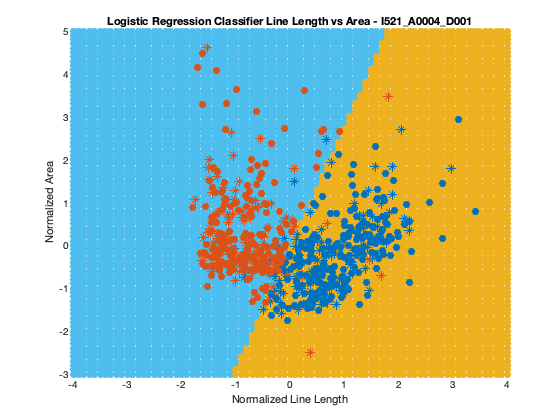
\includegraphics [width=5in]{jalp_hw4_05.png}
\begin{lstlisting}
%KNN plot
X = trainFeats_norm;
Y = cell2mat(train_data(:,1));

%KNN building
knn = fitcknn(X,Y, 'NumNeighbors', 1);

%grid classification
Ypred_grid = predict(knn, grid_norm);

yel = find(Ypred_grid(:,1)==1);
cya = find(Ypred_grid(:,1)==2);

%training index
hfo_train = find(Y(:,1)==2);
artif_train = find(Y(:,1)==1);

%testing points
X  = testFeats_norm;
Y_test = cell2mat(test_data(:,1));
Ypred_test_knn = predict(knn, X);

%testing index
hfo_test = find(Ypred_test_mnr(:,1)==2);
artif_test = find(Ypred_test_mnr(:,1)==1);
\end{lstlisting}
\begin{lstlisting}
figure();
scatter(grid_norm(yel,1), grid_norm(yel,2), 60,  'filled', 'MarkerFaceColor',[0.3010 0.7450 0.9330])
hold on
scatter(grid_norm(cya, 1), grid_norm(cya,2), 60, 'filled', 'MarkerFaceColor', [0.9290 0.6940 0.1250]) %HFO

%training set
scatter(trainFeats_norm(hfo_train,1), trainFeats_norm(hfo_train,2),'*', 'MarkerEdgeColor', [0 0.4470 0.7410])
scatter(trainFeats_norm(artif_train, 1), trainFeats_norm(artif_train,2), '*', 'MarkerEdgeColor', [0.8500 0.3250 0.0980])

%testing set
scatter(testFeats_norm(hfo_test,1), testFeats_norm(hfo_test,2), 60, 'filled' ,'MarkerFaceColor', [0 0.4470 0.7410])
scatter(testFeats_norm(artif_test, 1), testFeats_norm(artif_test,2), 60, 'filled','MarkerFaceColor', [0.8500 0.3250 0.0980])

title('KNN Line Length vs Area - I521\_A0004\_D001')
xlabel('Normalized Line Length')
ylabel('Normalized Area')
xlim([-4,4])
ylim([-3,5])
\end{lstlisting}


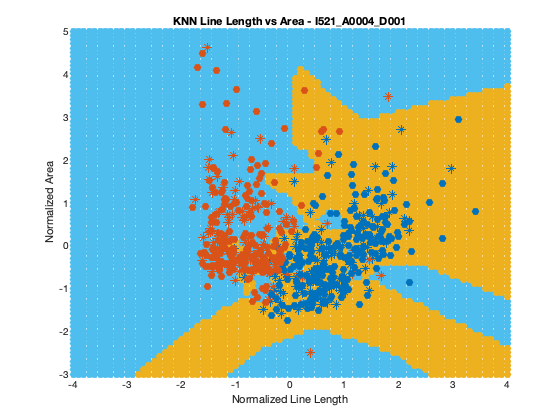
\includegraphics [width=5in]{jalp_hw4_06.png}
\begin{lstlisting}
%SVN plot
X = trainFeats_norm;
Y = cell2mat(train_data(:,1));

%SVN model building
svmodel = fitcsvm(X,Y, 'KernelFunction','rbf');


%grid classification
Ypred_grid = predict(svmodel, grid_norm);

yel = find(Ypred_grid(:,1)==1);
cya = find(Ypred_grid(:,1)==2);

%training index
hfo_train = find(Y(:,1)==2);
artif_train = find(Y(:,1)==1);

%testing points
X  = testFeats_norm;
Y_test = cell2mat(test_data(:,1));
Ypred_test_knn = predict(svmodel, X);

%testing index
hfo_test = find(Ypred_test_mnr(:,1)==2);
artif_test = find(Ypred_test_mnr(:,1)==1);
\end{lstlisting}
\begin{lstlisting}
figure();
scatter(grid_norm(yel,1), grid_norm(yel,2), 60,  'filled', 'MarkerFaceColor',[0.3010 0.7450 0.9330])
hold on
scatter(grid_norm(cya, 1), grid_norm(cya,2), 60, 'filled', 'MarkerFaceColor', [0.9290 0.6940 0.1250]) %HFO

%training set
scatter(trainFeats_norm(hfo_train,1), trainFeats_norm(hfo_train,2),'*', 'MarkerEdgeColor', [0 0.4470 0.7410])
scatter(trainFeats_norm(artif_train, 1), trainFeats_norm(artif_train,2), '*', 'MarkerEdgeColor', [0.8500 0.3250 0.0980])

%testing set
scatter(testFeats_norm(hfo_test,1), testFeats_norm(hfo_test,2), 60, 'filled' ,'MarkerFaceColor', [0 0.4470 0.7410])
scatter(testFeats_norm(artif_test, 1), testFeats_norm(artif_test,2), 60, 'filled','MarkerFaceColor', [0.8500 0.3250 0.0980])

title('SVN Line Length vs Area - I521\_A0004\_D001')
xlabel('Normalized Line Length')
ylabel('Normalized Area')
xlim([-4,4])
ylim([-3,5])
\end{lstlisting}


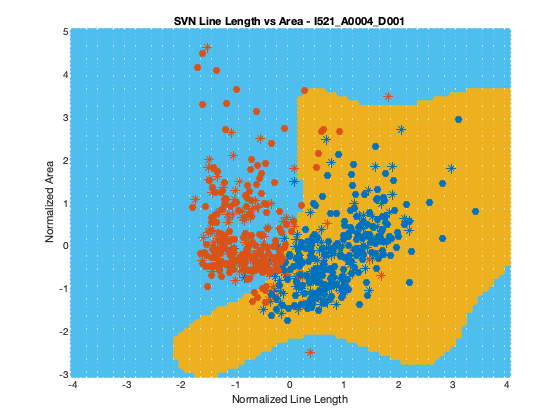
\includegraphics [width=5in]{jalp_hw4_07.png}

 \item In a few sentences, report some observations about the three
 plots, especially similarities and differences between them. Which
 of these has overfit the data the most? Which has underfit the data
 the most? (3 pts) \\


\textbf{Answer 3.6:}

In the three plots we can se the varying levels of agression of fitting the data. The KNN classifier with k=1 looks the most agressive and overfit where it tries to get regions for even single points. This overfitting has caused it to wrongly classify the most number of testing samples. $\\$ The SVN is the next most agressive classifier where it has tried to reach for most possible points in one closed boundary. We can visually also see why it has the least training error. $\\$. The Logistic regression classifier seems like underfit where several training and testing samples are classified incorrectly.

\end{enumerate}
\section{Cross-Validation (17 pts)} In this section, you will
investigate the importance of cross-validation, which is essential
for choosing the tunable parameters of a model (as opposed to the
internal parameters the the classifier ``learns'' by itself on the
training data).
\begin{enumerate}
 \item Since you cannot do any validation on the testing set, you'll
 have to split up the training set. One way of doing this is to
 randomly split it into $k$ unique ``folds,'' with roughly the same
 number of samples ($n/k$ for $n$ total training samples) in each
 fold, training on $k-1$ of the folds and doing predictions on the
 remaining one.
 In this section, you will do 10-fold cross-validation, so create a
 cell array\footnote{A cell array is slightly different from a
 normal Matlab numeric array in that it can hold elements of
 variable size (and type), for example \texttt{folds\{1\} = [1 3 6]; folds\{2\}
 = [2 5]; folds\{3\} = [4 7];}.} \texttt{folds} that contains 10
 elements, each of which is itself an array of the indices of
 training samples in that fold. You may find the \texttt{randperm}
 function useful for this.
 Using the command \texttt{length(unique([folds\{:\}]))}, show that
 you have 200 unique sample indices (i.e. there are no repeats
 between folds). (2 pts) \\


\textbf{Answer 4.1:}

\begin{lstlisting}
%creating a randon order of training sample indices
rand_ord = randperm(200);
%reshaping it in to a 10 cell containing 20 unique indices
rand_ord = reshape(rand_ord, 10, []);
knn_folds = num2cell(rand_ord, 2);

number_of_unique_indices = length(unique([knn_folds{:}]))
\end{lstlisting}

\color{lightgray} \begin{lstlisting}
number_of_unique_indices =

   200

\end{lstlisting} \color{black}

 \item Train a new $k$-NN model (still using the default parameters)
 on the folds you just created. Predict the labels for each fold
 using a classifier trained on all the other folds. After running
 through all the folds, you will have label predictions for each
 training sample.
  \begin{enumerate}
   \item Compute the error (called the validation error) of these
   predictions. (3 pts) \\


\textbf{Answer 4.2a:}

\begin{lstlisting}
%Calculating the validation error for each fold

idx = 1:200;

for i =1:10

    %finding the index of training set
    train_idx = idx(~ismember(idx,knn_folds{i,1}));

    %training model for folds other than i
    X = trainFeats_norm(train_idx, :);
    Y = cell2mat(train_data(train_idx,1));
    knn = fitcknn(X,Y, 'NumNeighbors', 1);

    %val set features
    X_val = trainFeats_norm(knn_folds{i,1},:);
    Y_val = cell2mat(train_data(knn_folds{i,1},1));

    %Calculating error
    Ypred_train = predict(knn, X_val);
    train_error = size(find(Ypred_train~=Y_val),1)/size(Y_val,1);

    %saving error in cell array
    knn_folds{i,2} = train_error;

end
\end{lstlisting}
The average validation error for all folds is
\begin{lstlisting}
avg_val_error = mean([knn_folds{:,2}])
\end{lstlisting}

\color{lightgray} \begin{lstlisting}
avg_val_error =

    0.1800

\end{lstlisting} \color{black}

\item How does this error compare (lower,
   higher, the same?) to the error you found in question 3.3? Does
   it make sense? (2 pts) \\


\textbf{Answer 4.2b:}

The average validation error varies everytime the folds were re- radomised, which is expected. The values I got were 15.5\%, 18\%, 16\% etc, which were all around the value of the testing error for K-nn got in Q3.3, 17.86\% and all of which are higher than the 0\% got as the training error. Both these results are as expected as by training the model on data from other folds and predicting the value of a given fold, this is similar to training using the complete training set and predicting the testing error. As the model was trained in a different set of data from the validation fold, the validation error was non-zero and was close to the values for testing error in Q3.3.

  \end{enumerate}
 \item Create a parameter space for your $k$-NN model by setting a
 vector of possible $k$ values from 1 to 30. For each values of $k$,
 calculate the validation error and average training error over the
 10 folds.
  \begin{enumerate}
   \item Plot the training and validation error values over the
   values of $k$, using the formatting string \texttt{'b-o'} for the
   validation error and \texttt{'r-o'} for the training error. (4
   pts) \\


\textbf{Answer 4.3a:}

\begin{lstlisting}
%Calculating validation and training error for differnt values of k
knn_k = 1:30;
val_error_mul_k = zeros(1,30);
train_error_mul_k = zeros(1,30);

for k = knn_k

    for i =1:10

        %finding the index of training set
        train_idx = idx(~ismember(idx,knn_folds{i,1}));

        %training model for folds other than i
        X = trainFeats_norm(train_idx, :);
        Y = cell2mat(train_data(train_idx,1));
        knn = fitcknn(X,Y, 'NumNeighbors', k); %varrying k

        %Calculating training error
        Ypred_train = predict(knn, X);
        train_error = size(find(Ypred_train~=Y),1)/size(Y,1);

        %val set features
        X_val = trainFeats_norm(knn_folds{i,1},:);
        Y_val = cell2mat(train_data(knn_folds{i,1},1));

        %Calculating validation error
        Ypred_val = predict(knn, X_val);
        val_error = size(find(Ypred_val~=Y_val),1)/size(Y_val,1);

        %saving error in cell array
        knn_folds{i,2+k} = [train_error, val_error];

    end

    %Calculating average val and training error for each k
    temp_ = [knn_folds{:,2+k}];
    temp_ = reshape(temp_,2,[])';

    train_error_mul_k(k) = mean(temp_(:,1));
    val_error_mul_k(k) = mean(temp_(:,2));
end
\end{lstlisting}
\begin{lstlisting}
%plotting errors against k
figure();
plot(knn_k,train_error_mul_k*100, 'r-o')
hold on
plot(knn_k,val_error_mul_k*100, 'b-o')
title('Training and Validation error for changing k - I521\_A0004\_D001')
xlabel('k values')
ylabel('Percentage error')
legend('Training error', 'Validation error')
\end{lstlisting}


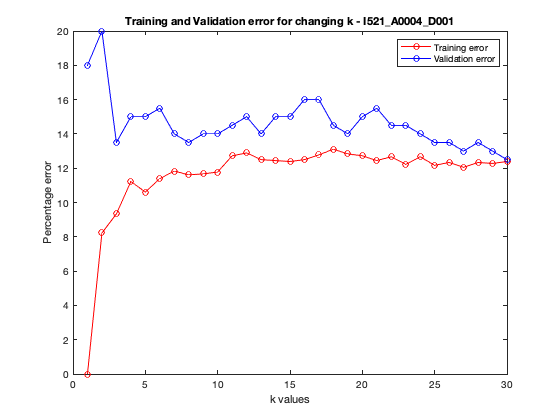
\includegraphics [width=5in]{jalp_hw4_08.png}

\item What is the optimal $k$ value and its training and testing error?
(1 pts) \\


\textbf{Answer 4.3b:}

As we increase the value of $k$ from 1:30 the validation error decreases and the traning error increases to reach stable values. The optimal k would be the one that gives the minimum value for the both the training and the validation errore. $\\$. Based on the graph, choosing a k from 26-30 should give similar results. I will choose a k=29 as the trend of error seems to be at the lowest point and the model will be more stable with new test data for a high k. With the current randomization of folds I get a validation error of 12.5\% and a training error of 12.28\%

   \item Explain why $k$-NN generally overfits less with higher
   values of $k$. (2 pts) \\


\textbf{Answer 4.3c:}

For smaller values of k the classifier is only looking a 1 nearest neighbor and so is very aggresive in fitting to every point in the training set. This causes an overfit. As k increases, the number of nearest neighbors considered increses and hence this smoothens fit and removed the micro level jaggednes of the classification boundary. As k increases we start seeing more of an average over several points which prevents overfitting and gives a more generic fit to the data.

  \end{enumerate}
 \item
  \begin{enumerate}
   \item Using your optimal value for $k$ from CV, calculate the
   $k$-NN model's \textit{testing} error. (1 pts) \\


\textbf{Answer 4.4a:}

\begin{lstlisting}
%Calculating testing error for optimal k
k = 29;
X = trainFeats_norm;
Y = cell2mat(train_data(:,1));
knn = fitcknn(X,Y, 'NumNeighbors', k);

X_test  = testFeats_norm;
Y_test = cell2mat(test_data(:,1));
Ypred_test = predict(knn, X_test);

test_error_opt = size(find(Ypred_test~=Y_test),1)/size(Y_test,1)
\end{lstlisting}

\color{lightgray} \begin{lstlisting}
test_error_opt =

    0.1143

\end{lstlisting} \color{black}
With a $k$ of 29, the testing error is 11.43\%

\item How does this
   model's testing error compare to the $k$-NN model
   you trained in question 3.3? Is it the best of the three models
   you trained in Section 3? (2 pts) \\


\textbf{Answer 4.4b:}

The testing error with $k$=29 is 11.43\% while that with $k$=1 in Q3.3 was 17.86\%, so the testing error has dropped with the increase in $k$. \%\ensuremath{\backslash}\ensuremath{\backslash}\% Comparing to the errors calculated in the other models, the logistic regression gave an error of 13.33\% and the SVN gave an error of 11.43\% for the the testing data. The optimised \%k\% has shown better results than the older $k$-NN model and the logistic regression model and has the same error as the SVM classifier.

  \end{enumerate}
\end{enumerate}




\end{document}
    
